\documentclass[aspectratio=169]{beamer}
\usetheme{default}\usecolortheme{whale}
\usepackage{booktabs}\usepackage{amsmath}\usepackage{graphicx}\usepackage{tikz}
\definecolor{best}{RGB}{0,90,200}\newcommand{\bb}[1]{\textcolor{best}{\textbf{#1}}}
\setbeamertemplate{navigation symbols}{}
\setbeamerfont{frametitle}{size=\large}
\title{Bitcoin Forecasting with VLA --- Results}\date{}
\begin{document}
\frame{\titlepage}
\begin{frame}{1. Overview}
\small
\textbf{Task:} Qwen3-VL (frozen) + flow-matching action head $\to$ next 12 hourly BTC candles.
Walk-forward 6-fold (2020--2025), BTC-only metrics, 0.1\% slippage. $k$ = holding horizon.
\vspace{.5ex}
\begin{center}\begin{tabular}{llll}
\toprule
Model & Head & Norm & Assets \\ \midrule
v14 & DiT & no & BTC+ETH+XRP (read-off) \\
v15\_btc & DiT & yes & BTC \\
v15\_multi & DiT & yes & BTC+ETH+XRP \\
v16\_msat\_btc & MSAT & yes & BTC \\
v16\_msat & MSAT & yes & BTC+ETH+XRP \\
v16\_msat\_v14 & MSAT & no & BTC+ETH+XRP (read-off) \\ \midrule
Kronos & pretrained & --- & BTC (fold6 only) \\
macro & DiT & yes & BTC+S\&P/bonds (2-fold) \\
\bottomrule
\end{tabular}\end{center}
\footnotesize DiT = cross-attention; MSAT = multi-stream joint attention (RLDX). B\&H: $+7.2\%$ (6-fold), $-5.3\%$ (fold6).
\end{frame}
\begin{frame}{Trading strategies}
\small
\textbf{Signal:} from the predicted candles, compute the expected move over horizon $k$: $\hat{m}=\hat{p}_{t+k}/p_t-1$.
Trade only if $|\hat{m}|>\theta$ (confidence gate, $\theta\in\{0.1,0.3,0.5,1.0\}\%$).
\vspace{.6ex}
\begin{center}\begin{tabular}{ll}
\toprule
Strategy & Position rule \\ \midrule
\textbf{Long-only} & long if $\hat{m}>\theta$, else flat (never short) \\
\textbf{Long-short} & long if $\hat{m}>\theta$; short if $\hat{m}<-\theta$; else flat \\
\textbf{Magnitude} & size $=\mathrm{clip}(\hat{m}/s,-1,1)$ (scaled by predicted size) \\
\bottomrule
\end{tabular}\end{center}
\vspace{.6ex}
\textbf{Backtest:} $k$-slot overlapping --- capital split into $k$ slots ($1/k$ each), enter every step, hold $k$ steps (avoids leverage inflation from stride-1 overlap). \textbf{Slippage 0.1\%} (Binance) per trade.
\vspace{.4ex}
\textbf{Metrics:} ret = principal return; AER = excess vs buy\&hold; MDD = max drawdown; DA = directional accuracy.
\end{frame}
\begin{frame}{How a trade works \& the $k$-slot backtest}
\small
\textbf{(1) Signal $\to$ enter $\to$ hold $k$ bars $\to$ exit.} At bar $t$ predict $k$ ahead; expected move $\hat m=\hat p_{t+k}/p_t-1$. Trade only if $|\hat m|>\theta$.
\begin{center}
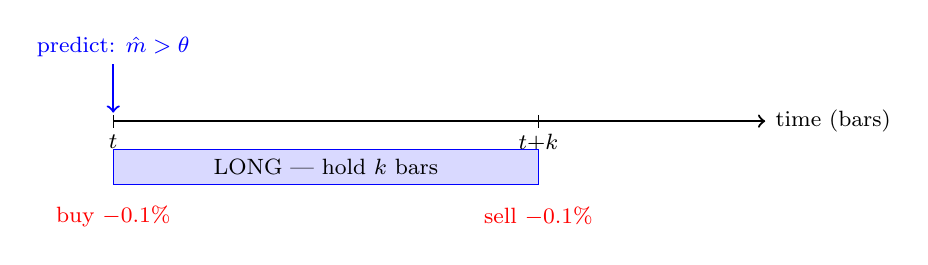
\begin{tikzpicture}[scale=0.9]
\draw[->,thick] (0,0)--(9.2,0) node[right]{\footnotesize time (bars)};
\foreach \x/\l in {0/{$t$},6/{$t{+}k$}} {\draw (\x,0.09)--(\x,-0.09); \node[below] at (\x,-0.05){\footnotesize \l};}
\node[align=center,blue] at (0,1.05){\footnotesize predict: $\hat m>\theta$};
\draw[->,thick,blue] (0,0.8)--(0,0.12);
\draw[fill=blue!15,draw=blue] (0,-0.9) rectangle (6,-0.4);
\node at (3,-0.65){\footnotesize LONG --- hold $k$ bars};
\node[red] at (0,-1.35){\footnotesize buy $-0.1\%$};
\node[red] at (6,-1.35){\footnotesize sell $-0.1\%$};
\end{tikzpicture}
\end{center}
\vspace{-0.5ex}
\textbf{(2) $k$-slot overlap.} A new signal every bar $\Rightarrow$ up to $k$ trades open at once. Capital is split into $k$ slots ($1/k$ each) so total exposure $\le100\%$ (no leverage from stride-1 overlap).
\begin{center}
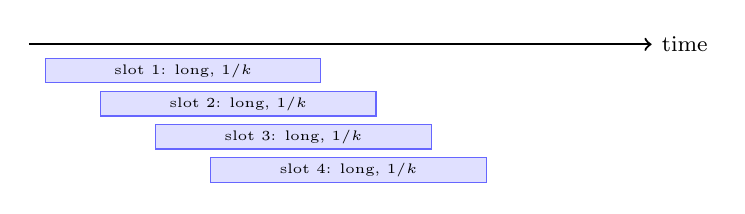
\begin{tikzpicture}[scale=0.7]
\draw[->,thick] (-0.3,0.7)--(11,0.7) node[right]{\footnotesize time};
\foreach \i/\n in {0/1,1/2,2/3,3/4}{
  \draw[fill=blue!12,draw=blue!60] (\i, -\i*0.6) rectangle (\i+5,-\i*0.6+0.45);
  \node[font=\tiny] at (\i+2.5,-\i*0.6+0.22){slot \n: long, $1/k$};
}
\end{tikzpicture}
\end{center}
\vspace{-0.5ex}
\footnotesize Combined equity curve $\to$ ret (principal return), AER (excess vs B\&H), MDD.
\end{frame}
\begin{frame}{Why target normalisation? (v14 raw $\to$ v15+ normalised)}
\small
\textbf{Target} = per-step delta log-return, then divided by each asset's training-range std.
\emph{v14} uses raw targets (no norm); \emph{v15/v16} normalise.
\vspace{.8ex}
\begin{enumerate}
\item \textbf{Flow-matching signal-to-noise:} raw hourly delta $\approx 0.1\%$, but the flow-matching noise is $\mathcal{N}(0,1)$. The tiny raw target is \emph{buried under the noise} $\Rightarrow$ the model barely learns it. Dividing by std makes the target unit-variance, matching the noise scale.
\item \textbf{Multi-asset balance:} BTC/ETH/XRP have different volatilities; per-asset std normalisation stops the high-vol asset from dominating the loss.
\item \textbf{Regime bias (empirical):} normalisation cut across-fold $\sigma(\text{Long\_ns})$ from \textbf{0.34} (v14) to \textbf{0.14--0.18} --- far less ``always-long / always-short'' memorisation.
\end{enumerate}
\vspace{.4ex}
\footnotesize At evaluation, predictions are un-normalised ($\times$ asset std) back to prices.
\end{frame}
\begin{frame}{2. Per-experiment DA \& Long\_ns ($k=1,3,6,12$, 6-fold avg)}
\small\textbf{Directional Accuracy (DA)} --- higher better\\[.3ex]
\begin{center}\begin{tabular}{llcccc}\toprule
Model & Setup & $k=1$ & $k=3$ & $k=6$ & $k=12$ \\ \midrule
v14 & DiT/raw/RO & 0.509 & 0.517 & \bb{0.527} & 0.525 \\
v15\_btc & DiT/norm/BTC & 0.507 & 0.511 & 0.517 & 0.517 \\
v15\_multi & DiT/norm/3A & 0.505 & 0.515 & 0.512 & 0.515 \\
v16\_msat\_btc & MSAT/norm/BTC & 0.511 & \bb{0.517} & 0.507 & 0.522 \\
v16\_msat & MSAT/norm/3A & 0.502 & 0.511 & 0.513 & 0.506 \\
v16\_msat\_v14 & MSAT/raw/RO & \bb{0.516} & 0.516 & 0.512 & \bb{0.532} \\
\bottomrule\end{tabular}\end{center}
\vspace{.4ex}\small\textbf{Long\_ns} (long-ratio, no-slippage) --- directional lean; near 1.0 = always-long\\[.3ex]
\begin{center}\begin{tabular}{llcccc}\toprule
Model & Setup & $k=1$ & $k=3$ & $k=6$ & $k=12$ \\ \midrule
v14 & DiT/raw/RO & 0.564 & 0.578 & 0.570 & 0.565 \\
v15\_btc & DiT/norm/BTC & 0.522 & 0.516 & 0.498 & 0.495 \\
v15\_multi & DiT/norm/3A & 0.555 & 0.590 & 0.616 & 0.648 \\
v16\_msat\_btc & MSAT/norm/BTC & 0.521 & 0.551 & 0.558 & 0.576 \\
v16\_msat & MSAT/norm/3A & 0.528 & 0.519 & 0.535 & 0.546 \\
v16\_msat\_v14 & MSAT/raw/RO & 0.477 & 0.441 & 0.399 & 0.361 \\
\bottomrule\end{tabular}\end{center}
\footnotesize (Regime memorisation shown by across-fold spread; see Conclusions.)\end{frame}
\begin{frame}{2b. Regime bias --- per-fold long-ratio ($k=6$, no slippage)}
\small Fraction of steps the model goes \emph{long} in each fold. Raw (no-norm) models swing to the extremes (all-long $\approx1$ / all-short $\approx0$) = \textbf{they memorise each fold's trend}. Normalisation keeps it moderate.\\[.6ex]
\begin{center}\resizebox{\ifdim\width>\linewidth\linewidth\else\width\fi}{!}{\begin{tabular}{llccccccc}\toprule
Model & Setup & F1 & F2 & F3 & F4 & F5 & F6 & $\sigma$ \\ \midrule
v14 & DiT/raw/RO & 1.00 & 0.18 & 0.44 & 0.75 & 0.92 & 0.12 & \textbf{0.343} \\
v15\_btc & DiT/norm/BTC & 0.71 & 0.39 & 0.29 & 0.58 & 0.72 & 0.30 & \bb{0.178} \\
v15\_multi & DiT/norm/3A & 0.83 & 0.41 & 0.48 & 0.72 & 0.68 & 0.57 & \bb{0.142} \\
v16\_msat\_btc & MSAT/norm/BTC & 0.74 & 0.46 & 0.45 & 0.58 & 0.60 & 0.52 & \bb{0.097} \\
v16\_msat & MSAT/norm/3A & 0.73 & 0.43 & 0.46 & 0.57 & 0.60 & 0.42 & \bb{0.111} \\
v16\_msat\_v14 & MSAT/raw/RO & 1.00 & 0.06 & 0.00 & 0.15 & 1.00 & 0.19 & \textbf{0.428} \\
\bottomrule\end{tabular}}\end{center}
\footnotesize $\sigma$ = across-fold std of long-ratio (regime-memorisation index). Raw v14 / v16\_msat\_v14 reach 0.00 and 1.00; normalised models stay $\approx0.3$--$0.7$.\end{frame}
\begin{frame}{3. Long-only strategy ($\theta=0.1\%$)}
\small 6-fold avg \quad each cell = \textbf{ret / AER}\\[.6ex]
\begin{center}\resizebox{\ifdim\width>\linewidth\linewidth\else\width\fi}{!}{\begin{tabular}{llcccc}\toprule
Model & Setup & $k=1$ & $k=3$ & $k=6$ & $k=12$ \\ \midrule
v14 & DiT/raw/RO & -0.264/-0.336 & -0.054/-0.124 & \bb{+0.033/-0.039} & +0.046/-0.024 \\
v15\_btc & DiT/norm/BTC & \bb{-0.161/-0.233} & -0.042/-0.112 & +0.023/-0.049 & +0.037/-0.033 \\
v15\_multi & DiT/norm/3A & -0.226/-0.297 & -0.078/-0.148 & -0.013/-0.085 & +0.024/-0.046 \\
v16\_msat\_btc & MSAT/norm/BTC & -0.193/-0.264 & -0.061/-0.130 & -0.007/-0.079 & +0.039/-0.032 \\
v16\_msat & MSAT/norm/3A & -0.205/-0.277 & -0.043/-0.113 & +0.016/-0.056 & +0.026/-0.044 \\
v16\_msat\_v14 & MSAT/raw/RO & -0.184/-0.255 & \bb{-0.028/-0.098} & +0.026/-0.046 & \bb{+0.057/-0.013} \\
\bottomrule\end{tabular}}\end{center}
\footnotesize ret=principal return, AER=excess return vs B\&H. $\theta$=confidence gate.\end{frame}
\begin{frame}{3. Long-only strategy ($\theta=0.3\%$)}
\small 6-fold avg \quad each cell = \textbf{ret / AER}\\[.6ex]
\begin{center}\resizebox{\ifdim\width>\linewidth\linewidth\else\width\fi}{!}{\begin{tabular}{llcccc}\toprule
Model & Setup & $k=1$ & $k=3$ & $k=6$ & $k=12$ \\ \midrule
v14 & DiT/raw/RO & -0.249/-0.321 & -0.053/-0.123 & \bb{+0.037/-0.035} & +0.048/-0.022 \\
v15\_btc & DiT/norm/BTC & -0.076/-0.147 & \bb{-0.005/-0.075} & +0.026/-0.046 & +0.038/-0.033 \\
v15\_multi & DiT/norm/3A & -0.106/-0.178 & -0.074/-0.144 & -0.016/-0.088 & +0.028/-0.042 \\
v16\_msat\_btc & MSAT/norm/BTC & -0.104/-0.176 & -0.055/-0.125 & +0.003/-0.069 & +0.034/-0.036 \\
v16\_msat & MSAT/norm/3A & \bb{-0.074/-0.145} & -0.041/-0.111 & +0.022/-0.050 & +0.026/-0.044 \\
v16\_msat\_v14 & MSAT/raw/RO & -0.156/-0.228 & -0.017/-0.087 & +0.030/-0.042 & \bb{+0.058/-0.012} \\
\bottomrule\end{tabular}}\end{center}
\footnotesize ret=principal return, AER=excess return vs B\&H. $\theta$=confidence gate.\end{frame}
\begin{frame}{3. Long-only strategy ($\theta=0.5\%$)}
\small 6-fold avg \quad each cell = \textbf{ret / AER}\\[.6ex]
\begin{center}\resizebox{\ifdim\width>\linewidth\linewidth\else\width\fi}{!}{\begin{tabular}{llcccc}\toprule
Model & Setup & $k=1$ & $k=3$ & $k=6$ & $k=12$ \\ \midrule
v14 & DiT/raw/RO & -0.230/-0.301 & -0.047/-0.117 & +0.035/-0.037 & +0.049/-0.022 \\
v15\_btc & DiT/norm/BTC & \bb{-0.033/-0.104} & \bb{+0.011/-0.059} & \bb{+0.040/-0.032} & +0.035/-0.035 \\
v15\_multi & DiT/norm/3A & -0.053/-0.124 & -0.046/-0.116 & -0.026/-0.098 & +0.031/-0.039 \\
v16\_msat\_btc & MSAT/norm/BTC & -0.052/-0.123 & -0.043/-0.113 & +0.013/-0.059 & +0.035/-0.035 \\
v16\_msat & MSAT/norm/3A & -0.045/-0.116 & -0.017/-0.087 & +0.027/-0.045 & +0.028/-0.042 \\
v16\_msat\_v14 & MSAT/raw/RO & -0.139/-0.210 & -0.014/-0.084 & +0.030/-0.042 & \bb{+0.059/-0.012} \\
\bottomrule\end{tabular}}\end{center}
\footnotesize ret=principal return, AER=excess return vs B\&H. $\theta$=confidence gate.\end{frame}
\begin{frame}{3. Long-only strategy ($\theta=1.0\%$)}
\small 6-fold avg \quad each cell = \textbf{ret / AER}\\[.6ex]
\begin{center}\resizebox{\ifdim\width>\linewidth\linewidth\else\width\fi}{!}{\begin{tabular}{llcccc}\toprule
Model & Setup & $k=1$ & $k=3$ & $k=6$ & $k=12$ \\ \midrule
v14 & DiT/raw/RO & -0.165/-0.236 & -0.035/-0.105 & \bb{+0.035/-0.037} & +0.050/-0.020 \\
v15\_btc & DiT/norm/BTC & \bb{-0.003/-0.075} & \bb{+0.007/-0.063} & +0.026/-0.046 & +0.030/-0.040 \\
v15\_multi & DiT/norm/3A & -0.005/-0.076 & -0.017/-0.086 & -0.014/-0.086 & +0.024/-0.047 \\
v16\_msat\_btc & MSAT/norm/BTC & -0.024/-0.095 & -0.014/-0.083 & +0.013/-0.059 & +0.036/-0.035 \\
v16\_msat & MSAT/norm/3A & -0.006/-0.078 & -0.003/-0.073 & +0.015/-0.057 & +0.029/-0.042 \\
v16\_msat\_v14 & MSAT/raw/RO & -0.125/-0.197 & -0.011/-0.081 & +0.034/-0.038 & \bb{+0.059/-0.011} \\
\bottomrule\end{tabular}}\end{center}
\footnotesize ret=principal return, AER=excess return vs B\&H. $\theta$=confidence gate.\end{frame}
\begin{frame}{3. Long-short strategy ($\theta=0.1\%$)}
\small 6-fold avg \quad each cell = \textbf{ret / AER}\\[.6ex]
\begin{center}\resizebox{\ifdim\width>\linewidth\linewidth\else\width\fi}{!}{\begin{tabular}{llcccc}\toprule
Model & Setup & $k=1$ & $k=3$ & $k=6$ & $k=12$ \\ \midrule
v14 & DiT/raw/RO & -0.438/-0.509 & \bb{-0.127/-0.197} & \bb{+0.007/-0.065} & +0.026/-0.045 \\
v15\_btc & DiT/norm/BTC & \bb{-0.323/-0.394} & -0.139/-0.209 & -0.031/-0.103 & +0.003/-0.067 \\
v15\_multi & DiT/norm/3A & -0.376/-0.447 & -0.162/-0.232 & -0.057/-0.129 & -0.003/-0.074 \\
v16\_msat\_btc & MSAT/norm/BTC & -0.339/-0.410 & -0.144/-0.214 & -0.057/-0.129 & +0.014/-0.057 \\
v16\_msat & MSAT/norm/3A & -0.365/-0.436 & -0.130/-0.200 & -0.026/-0.098 & -0.011/-0.082 \\
v16\_msat\_v14 & MSAT/raw/RO & -0.383/-0.455 & -0.132/-0.202 & -0.041/-0.113 & \bb{+0.027/-0.043} \\
\bottomrule\end{tabular}}\end{center}
\footnotesize ret=principal return, AER=excess return vs B\&H. $\theta$=confidence gate.\end{frame}
\begin{frame}{3. Long-short strategy ($\theta=0.3\%$)}
\small 6-fold avg \quad each cell = \textbf{ret / AER}\\[.6ex]
\begin{center}\resizebox{\ifdim\width>\linewidth\linewidth\else\width\fi}{!}{\begin{tabular}{llcccc}\toprule
Model & Setup & $k=1$ & $k=3$ & $k=6$ & $k=12$ \\ \midrule
v14 & DiT/raw/RO & -0.412/-0.483 & -0.121/-0.191 & \bb{+0.011/-0.061} & \bb{+0.029/-0.042} \\
v15\_btc & DiT/norm/BTC & -0.180/-0.252 & \bb{-0.076/-0.146} & -0.008/-0.080 & +0.016/-0.055 \\
v15\_multi & DiT/norm/3A & -0.171/-0.242 & -0.127/-0.197 & -0.050/-0.122 & +0.005/-0.065 \\
v16\_msat\_btc & MSAT/norm/BTC & -0.167/-0.239 & -0.109/-0.179 & -0.034/-0.106 & +0.013/-0.057 \\
v16\_msat & MSAT/norm/3A & \bb{-0.144/-0.215} & -0.100/-0.170 & -0.002/-0.074 & -0.004/-0.074 \\
v16\_msat\_v14 & MSAT/raw/RO & -0.318/-0.389 & -0.107/-0.177 & -0.036/-0.108 & +0.027/-0.043 \\
\bottomrule\end{tabular}}\end{center}
\footnotesize ret=principal return, AER=excess return vs B\&H. $\theta$=confidence gate.\end{frame}
\begin{frame}{3. Long-short strategy ($\theta=0.5\%$)}
\small 6-fold avg \quad each cell = \textbf{ret / AER}\\[.6ex]
\begin{center}\resizebox{\ifdim\width>\linewidth\linewidth\else\width\fi}{!}{\begin{tabular}{llcccc}\toprule
Model & Setup & $k=1$ & $k=3$ & $k=6$ & $k=12$ \\ \midrule
v14 & DiT/raw/RO & -0.384/-0.456 & -0.108/-0.178 & +0.008/-0.064 & +0.027/-0.043 \\
v15\_btc & DiT/norm/BTC & -0.098/-0.169 & \bb{-0.031/-0.101} & \bb{+0.013/-0.059} & +0.021/-0.050 \\
v15\_multi & DiT/norm/3A & -0.082/-0.153 & -0.085/-0.155 & -0.053/-0.125 & +0.008/-0.062 \\
v16\_msat\_btc & MSAT/norm/BTC & -0.096/-0.167 & -0.066/-0.136 & -0.010/-0.082 & +0.019/-0.051 \\
v16\_msat & MSAT/norm/3A & \bb{-0.053/-0.125} & -0.044/-0.114 & +0.004/-0.068 & +0.006/-0.064 \\
v16\_msat\_v14 & MSAT/raw/RO & -0.277/-0.348 & -0.092/-0.162 & -0.023/-0.095 & \bb{+0.028/-0.042} \\
\bottomrule\end{tabular}}\end{center}
\footnotesize ret=principal return, AER=excess return vs B\&H. $\theta$=confidence gate.\end{frame}
\begin{frame}{3. Long-short strategy ($\theta=1.0\%$)}
\small 6-fold avg \quad each cell = \textbf{ret / AER}\\[.6ex]
\begin{center}\resizebox{\ifdim\width>\linewidth\linewidth\else\width\fi}{!}{\begin{tabular}{llcccc}\toprule
Model & Setup & $k=1$ & $k=3$ & $k=6$ & $k=12$ \\ \midrule
v14 & DiT/raw/RO & -0.280/-0.352 & -0.094/-0.164 & +0.005/-0.067 & +0.031/-0.040 \\
v15\_btc & DiT/norm/BTC & -0.021/-0.093 & -0.017/-0.087 & \bb{+0.007/-0.065} & +0.021/-0.050 \\
v15\_multi & DiT/norm/3A & -0.013/-0.085 & -0.038/-0.108 & -0.020/-0.092 & +0.016/-0.054 \\
v16\_msat\_btc & MSAT/norm/BTC & -0.033/-0.104 & -0.026/-0.096 & -0.002/-0.074 & +0.024/-0.046 \\
v16\_msat & MSAT/norm/3A & \bb{-0.004/-0.076} & \bb{-0.007/-0.077} & +0.007/-0.065 & +0.017/-0.054 \\
v16\_msat\_v14 & MSAT/raw/RO & -0.201/-0.272 & -0.085/-0.155 & -0.010/-0.082 & \bb{+0.038/-0.032} \\
\bottomrule\end{tabular}}\end{center}
\footnotesize ret=principal return, AER=excess return vs B\&H. $\theta$=confidence gate.\end{frame}
\begin{frame}{3. Magnitude strategy}
\small 6-fold avg \quad each cell = \textbf{ret / AER}\\[.6ex]
\begin{center}\resizebox{\ifdim\width>\linewidth\linewidth\else\width\fi}{!}{\begin{tabular}{llcccc}\toprule
Model & Setup & $k=1$ & $k=3$ & $k=6$ & $k=12$ \\ \midrule
v14 & DiT/raw/RO & -0.341/-0.412 & -0.083/-0.153 & \bb{+0.013/-0.059} & \bb{+0.035/-0.035} \\
v15\_btc & DiT/norm/BTC & \bb{-0.263/-0.334} & \bb{-0.076/-0.146} & -0.008/-0.080 & +0.019/-0.051 \\
v15\_multi & DiT/norm/3A & -0.314/-0.385 & -0.124/-0.193 & -0.045/-0.117 & +0.012/-0.059 \\
v16\_msat\_btc & MSAT/norm/BTC & -0.281/-0.353 & -0.112/-0.182 & -0.034/-0.106 & +0.015/-0.055 \\
v16\_msat & MSAT/norm/3A & -0.289/-0.360 & -0.100/-0.170 & -0.006/-0.079 & +0.006/-0.064 \\
v16\_msat\_v14 & MSAT/raw/RO & -0.357/-0.428 & -0.116/-0.186 & -0.030/-0.102 & +0.028/-0.042 \\
\bottomrule\end{tabular}}\end{center}
\footnotesize ret=principal return, AER=excess return vs B\&H. $\theta$=confidence gate.\end{frame}
\begin{frame}{4. Best strategy per model --- 6-fold average}
\small For each model, the setup with the highest \textbf{ret} (over all strategies/$\theta$/$k$):\\[.6ex]
\begin{center}\resizebox{\ifdim\width>\linewidth\linewidth\else\width\fi}{!}{\begin{tabular}{lllccc}\toprule
Model & Setup & Strategy & $k$ & ret & AER \\ \midrule
v14 & DiT/raw/RO & long-only $\theta1.0$ & 12 & +0.050 & -0.020 \\
v15\_btc & DiT/norm/BTC & long-only $\theta0.5$ & 6 & +0.040 & -0.032 \\
v15\_multi & DiT/norm/3A & long-only $\theta0.5$ & 12 & +0.031 & -0.039 \\
v16\_msat\_btc & MSAT/norm/BTC & long-only $\theta0.1$ & 12 & +0.039 & -0.032 \\
v16\_msat & MSAT/norm/3A & long-only $\theta1.0$ & 12 & +0.029 & -0.042 \\
v16\_msat\_v14 & MSAT/raw/RO & long-only $\theta1.0$ & 12 & \bb{+0.059} & -0.011 \\
\bottomrule\end{tabular}}\end{center}
\footnotesize All AER $<0$: even each model's best beats \emph{no} model past B\&H ($+7.2\%$). Best ret = \textbf{v16\_msat\_v14} $+5.9\%$ (long-only, $k{=}12$).\end{frame}
\begin{frame}{4. Both positive (ret \& AER)? --- only on fold6}
\small \textbf{6-fold average: \bb{ZERO}} setups have ret$>0$ \emph{and} AER$>0$ (nothing beats B\&H's $+7.2\%$).\\
\textbf{fold6} (falling market, B\&H$=-5.3\%$) --- top setups with both positive (by AER):\\[.6ex]
\begin{center}\resizebox{\ifdim\width>\linewidth\linewidth\else\width\fi}{!}{\begin{tabular}{lllccc}\toprule
Model & Strategy & $\theta$ & $k$ & ret & AER \\ \midrule
\bb{Kronos} & long-short & 0.3 & 12 & \bb{+0.125} & \bb{+0.178} \\
\bb{Kronos} & long-short & 0.1 & 12 & \bb{+0.119} & \bb{+0.171} \\
v15\_multi & long-only & 1.0 & 3 & +0.014 & +0.064 \\
v15\_btc & long-only & 1.0 & 1 & +0.013 & +0.062 \\
v15\_btc & long-short & 1.0 & 3 & +0.011 & +0.060 \\
v16\_msat & long-short & 1.0 & 3 & +0.010 & +0.060 \\
v15\_btc & long-short & 1.0 & 1 & +0.009 & +0.058 \\
\bottomrule\end{tabular}}\end{center}
\footnotesize Our models: tiny positives only at high gate; \textbf{Kronos dominates} (matches slide~5's max-over-$\theta$).\end{frame}
\begin{frame}{5. Our models vs Kronos (fold6, clean OOS)}
\small Best strategy return (max over long/short, all $\theta$) on fold6:\\[.3ex]
\begin{center}\begin{tabular}{lcccc}\toprule
Model & $k=1$ & $k=3$ & $k=6$ & $k=12$ \\ \midrule
v14 & -0.099 & -0.059 & -0.024 & -0.010 \\
v15\_btc & \bb{+0.013} & +0.011 & -0.014 & +0.003 \\
v15\_multi & -0.004 & +0.014 & -0.036 & -0.043 \\
v16\_msat\_btc & -0.004 & -0.070 & -0.011 & -0.028 \\
v16\_msat & +0.004 & +0.010 & -0.004 & +0.004 \\
v16\_msat\_v14 & -0.110 & -0.028 & -0.028 & -0.003 \\
\bb{Kronos} & +0.002 & \bb{+0.036} & \bb{+0.059} & \bb{+0.125} \\
\midrule B\&H & -0.050 & -0.049 & -0.053 & -0.052 \\
\bottomrule\end{tabular}\end{center}
\footnotesize Kronos (June-2024 cutoff) is only valid on fold6 (2025). It is the \textbf{only positive} model, widening with $k$.\end{frame}
\begin{frame}{6. Macro experiments (BTC + S\&P/bonds, 2-fold)}
\small Separate dataset (market-hours aligned, 52 test samples). DA / ret / AER / LO-best by $k$:\\[.3ex]
\begin{center}\footnotesize\begin{tabular}{lcccc }\toprule
Experiment ($k{=}6$) & DA & ret & AER & LO best \\ \midrule
baseline (BTC only) & 0.465 & \bb{-0.027} & \bb{+0.028} & -0.031 \\
BTC+TLT+SPY & \bb{0.472} & -0.029 & +0.026 & \bb{-0.021} \\
BTC+SPY+IEF & 0.363 & -0.051 & +0.005 & -0.036 \\
BTC+SPY+SHY & 0.419 & -0.047 & +0.008 & -0.028 \\
\bottomrule\end{tabular}\end{center}
\vspace{.5ex}\footnotesize \textbf{Adding S\&P/bonds does not improve BTC} --- DA near/below baseline, gains within noise (bonds corr $\approx0$, S\&P $\approx0.4$; only 2 folds).\end{frame}
\begin{frame}{7. Conclusions}
\small
\begin{enumerate}
\item \textbf{Normalisation cuts regime bias}: across-fold $\sigma$(Long\_ns) drops $0.34\to0.10$--$0.18$ (v14 memorises each fold's trend).
\item \textbf{v14's high average return is a mirage} (uptrend memorisation) --- worst on the clean fold6.
\item \textbf{Multi-asset does not help under DiT}; \textbf{MSAT partially rescues it} (joint attention), but stays below single-asset DiT.
\item \textbf{MSAT $>$ DiT only for multi-asset}; single-asset / read-off $\Rightarrow$ DiT wins.
\item \textbf{Macro (S\&P/bonds) does not help} BTC.
\item \textbf{Nothing is profitable \emph{and} beats B\&H} on 6-fold average; on fold6 \textbf{only Kronos} is positive.
\end{enumerate}
\vspace{.5ex}
\textbf{Best of ours: v15\_btc} (BTC-only, normalised, DiT) --- LO@0.5\% $+4.0\%$ vs B\&H $+7.2\%$.
\end{frame}
\end{document}